\documentclass[11pt,a4paper]{article}
\usepackage[utf8]{inputenc}
\usepackage[T1]{fontenc}
\usepackage[margin=2.5cm]{geometry}
\usepackage{graphicx}
\usepackage{booktabs}
\usepackage{amsmath}
\usepackage{hyperref}
\hypersetup{colorlinks=true, linkcolor=blue, urlcolor=blue, citecolor=blue}

\title{\textbf{Electricity Demand Forecasting in France}\\
\large A weather- and calendar-driven multi-output forecasting pipeline}
\author{Marcos Lahoz}
\date{\today}

\begin{document}
\maketitle

\begin{abstract}
We forecast half-hourly electricity demand for France, its 12 administrative
regions and 12 métropoles --- 25 series in total --- for the year 2022, using
only weather observations and calendar information. We compare three models of
increasing complexity (a seasonal climatology baseline, a multi-output neural
network and per-series gradient-boosted trees) under a strict temporal
validation protocol and the official challenge metric, the sum of the
per-series RMSE. Gradient boosting is the strongest model, reducing the
validation score by 39\% relative to the seasonal baseline.
\end{abstract}

\section{Introduction}
Short-term electricity demand forecasting is central to grid operation and
energy trading. This work addresses a data-challenge formulation: given
historical demand (2017--2021) and meteorological data, predict the demand of
2022 for 25 geographic series simultaneously. Models are scored with
\[
\text{score} = \sum_{s=1}^{25} \mathrm{RMSE}_s,
\]
the sum of the per-series root-mean-squared errors (lower is better). The same
quantity is used as the training loss of the neural network, so the model
optimises exactly the metric it is evaluated on.

\section{Data}
Three sources are provided: half-hourly demand for the 25 series
(2017--2021); the 2022 timestamps to predict; and three-hourly observations
from 40 Météo-France SYNOP stations distributed across the 12 regions
(2017--2022). The 12 métropole series only begin partway through the training
period, so the targets contain missing values; every stage of the pipeline is
therefore made NaN-aware. Each target is mapped to the weather of its region
(the national series uses the average across regions); stations are averaged
per region and the resulting signal is resampled from three-hourly to the
30-minute grid of the demand series.

\section{Methodology}

\subsection{Feature engineering}
All features are available for the 2022 horizon (no leakage from future
targets). \emph{Calendar} features are computed in French local time: cyclical
encodings of time-of-day, day-of-week and day-of-year, weekend and public
holiday flags, and a yearly trend. \emph{Weather} features include per-region
temperature, humidity, wind and pressure, heating- and cooling-degree
quantities (HDD/CDD), a national aggregate, and 24\,h/48\,h rolling
temperatures that capture the thermal inertia of demand.

\subsection{Validation protocol}
Because the data is a time series, we use a strictly chronological split:
models are trained on 2017--2020 and validated on the held-out year 2021. A
random split would leak future information and over-estimate performance.

\subsection{Models}
\begin{itemize}
  \item \textbf{Seasonal baseline} --- the historical mean demand for each
        (month, weekday, half-hour) cell; a strong, weather-free reference.
  \item \textbf{Neural network (MLP)} --- a two-hidden-layer perceptron with
        batch normalisation, dropout and Xavier initialisation, trained with
        mini-batches, early stopping, and the sum-of-RMSE loss (the challenge
        metric). The network predicts in standardised output space for stable
        optimisation while the loss is evaluated on the raw scale.
  \item \textbf{Gradient boosting} --- one histogram-based gradient-boosting
        regressor per series, each trained on the rows where its target is
        observed.
\end{itemize}

\section{Results}
Table~\ref{tab:results} and Figure~\ref{fig:comp} report the 2021 hold-out
performance. Both learned models beat the seasonal baseline, and gradient
boosting is clearly the best, lowering the challenge score from 11541 to 7037
(a 39\% reduction) and roughly halving the mean absolute error. The neural
network improves on the baseline but trails the trees, which handle the
non-linear temperature--demand relationship and the heterogeneous scales of
the 25 series particularly well.

\begin{table}[h]
\centering
\begin{tabular}{lrr}
\toprule
\textbf{Model} & \textbf{Challenge score} & \textbf{MAE} \\
\midrule
Seasonal baseline      & 11541.1 & 332.5 \\
MLP (PyTorch)          &  9834.9 & 321.0 \\
\textbf{Gradient boosting} & \textbf{7036.6} & \textbf{211.1} \\
\bottomrule
\end{tabular}
\caption{Performance on the 2021 hold-out year (sum of per-series RMSE; lower
is better).}
\label{tab:results}
\end{table}

\begin{figure}[h]
\centering
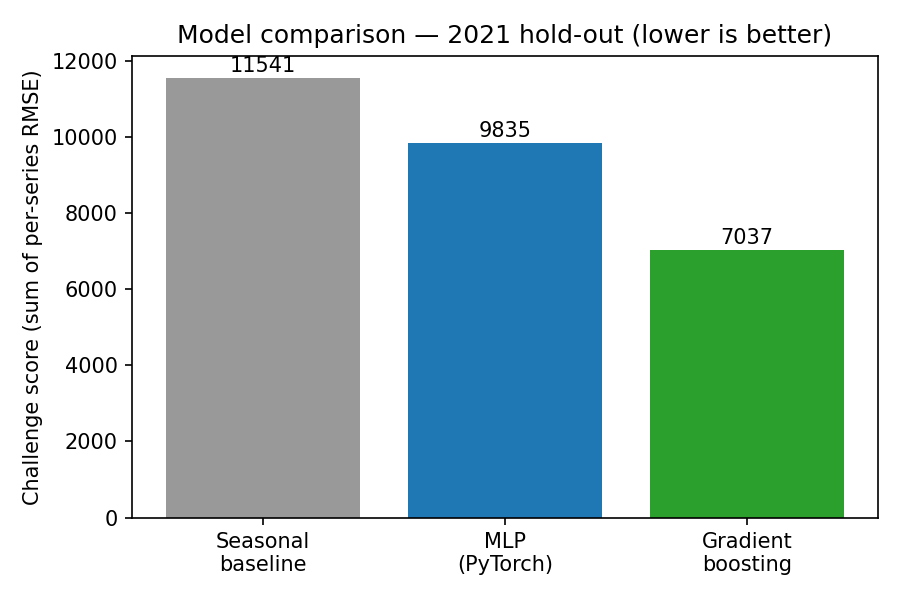
\includegraphics[width=0.72\textwidth]{figures/model_comparison.png}
\caption{Validation challenge score by model on the 2021 hold-out.}
\label{fig:comp}
\end{figure}

\section{Conclusion}
A compact pipeline built on temperature, calendar and degree-day features
predicts the 25 demand series well across France. Under an honest temporal
validation, per-series gradient boosting is the most accurate model and is used
to generate the 2022 submission. Natural extensions include population-weighted
national aggregation, lagged-demand features for shorter horizons, and a
boosting/neural ensemble.

\section*{Reproducibility}
The full code, models and instructions are available in the project repository.
Results reproduce with \texttt{python scripts/evaluate.py --raw-dir data/raw
--models baseline mlp gbm}.

\begin{thebibliography}{9}
\bibitem{synop} Météo-France. \emph{SYNOP observation data} (Données SYNOP
essentielles OMM).
\bibitem{sklearn} Pedregosa et al. \emph{Scikit-learn: Machine Learning in
Python}. JMLR, 2011 (HistGradientBoostingRegressor).
\bibitem{torch} Paszke et al. \emph{PyTorch: An Imperative Style,
High-Performance Deep Learning Library}. NeurIPS, 2019.
\end{thebibliography}

\end{document}
